\section{Projektstrukturplan}

\subsection{Zielbestimmung}
\subsubsection{Musskriterien}
Diese Kriterien müssen bis zum Projektende implementiert werden, damit das Projekt erfolgreich abgeschlossen ist.

\begin{enumerate}[leftmargin=2cm, label=\bfseries /MK\arabic*0/]
	\item Der Benutzer kann Karteikartensets erstellen, die Themen für eine Sammlung von Karteikarten darstellt.
	\item Der Benutzer kann Karteikarten zu einem Karteikartenset hinzufügen und löschen.
	\item Der Benutzer kann angeben, ob er eine Karteikarte richtig oder falsch beantwortet hat.
	\item\label{unicode} Unicode-Zeichen werden als Eingabe in den Karteikarten unterstützt.
	\item\label{keyboard} Beim Lernen mit den Karteikarten kann auch nur mit der Tastatur navigiert werden.
\end{enumerate}


\subsubsection{Wunschkriterien}
Diese Kriterien werden für das Projekt gewünscht, sind aber nicht zwingend erforderlich für ein erfolgreiches Projektende. Je nach Zeit und technisches Schwierigkeitsgrad wird versucht möglichst viele/wichtige Kriterien zu implementieren.

\begin{enumerate}[leftmargin=2cm, label=\bfseries /WK\arabic*0/]
	%\item Die Webseite wird zusätzlich auch für Mobilgeräte optimiert.
	\item Für jedes Karteikartenset werden Statistiken angezeigt (Erfolgsquote,...).
	\item Mathematische Ausdrücke werden dargestellt in natürlicher Form (z.b. \( e^{\frac{3}{4}\pi i}\))
	\item Die Antwortkarte kann in Form von Multiple Choice sein.
	\item Die zu lernenden Karten werden durch einen Algorithmus ausgewählt (z.B. Leitner System)
	\item Bilder können eingefügt werden.
	\item\label{export} Ein Karteikartenset kann vom Benutzer exportiert werden.
	%\item\label{katalog} Die Seite stellt ein Katalog von vorgefertigten Karteikartensets zur Verfügung.
	\item\label{share} Der Benutzer hat Option ein Karteikartenset mit einer anderen Person zu teilen.
	\item Ein (anderer) Benutzer kann das vom \ref{export} exportierte Karteikartenset in seinen Account importieren.
\end{enumerate}

\subsubsection{Abgrenzkriterien}
Diese Kriterien beschreiben die Grenzen des Projektes und sollen auf jeden Fall nicht implementiert werden.

\begin{enumerate}[leftmargin=2cm, label=\bfseries /AK\arabic*0/]
	\item Videos müssen nicht in die Karten eingebettet sein. (Sie können trotzdem einfach als Hyperlink eingefügt werden.)
	\item Die Webseite muss nicht offline funktionieren.
	\item Bei Verbindungsverlust muss der aktuelle Stand nicht zwischengespeichert werden.
\end{enumerate}



\newpage
\subsection{Produkteinsatz}
% in diesem Kapitel kann der Einsatz auch eingegrenzt werden

\subsubsection{Anwendungsbereiche}
Die Webseite richtet sich an Einzelpersonen, die Informationen lernen müssen, welches in das Schema "Frage" und "Antwort" eingeordnet werden kann.

\subsubsection{Zielgruppen}
\begin{enumerate}[leftmargin=2cm, label=\bfseries /ZG\arabic*0/]
	\item Die Webseite richtet sich an Personen, die eine neue Fremdsprache lernen wollen.
	\item Eine weitere Zielgruppe sind Schüler, die die Webseite begleitend zum Unterricht benutzen.
	\item Die letzte Gruppe sind Studenten, die die Webseite begleitend zum Studium benutzen.
\end{enumerate}


\subsubsection{Betriebsbedingungen}
Die Betriebsbedingungen beschreiben die physikalische Umgebung und tägliche Betriebszeit.\\

\noindent Das Projekt läuft auf einem Server, der JSP-Spezifikation unterstützt. Dieser kann entweder auf einem lokalen Computer oder in einem Rechenzentrum eines Server-Anbieters laufen. Da der Server-Verantwortlicher ein Student ist, ist der Server für ein Großteil des Tages in einen unbeaufsichtigten Betrieb. Außer für Wartungsarbeiten soll die Webseite rund um die Uhr erreichbar sein.

%\subsection{Produktübersicht}

\subsection{Produktdaten}
\subsubsection{Benutzer}
Zu dem angemeldeten Benutzer werden diese Daten dauerhaft gespeichert:
\begin{itemize}
	\item Benutzername
	\item E-Mail-Adresse
	\item Password
\end{itemize}

\subsubsection{Lernkartei}
Für jede einzelne Lernkartei werden diese Informationen gespeichert:
\begin{itemize}
	\item Inhalt der Frage
	\item Inhalt der Antwort
	\item Anzahl der richtigen und falschen Beantworten der Frage
	\item Zeitpunkt der letzten richtigen Beantwortung der Frage
\end{itemize}


\newgeometry{margin=2cm} % modify this if you need even more space
\begin{landscape}
\begin{center}
\subsection{Produktfunktionen}


\begin{tabulary}{1.35\textwidth}{|L|L|L|L|L|L|L|}
\hline 
\textbf{Anwendungsfall} & \textbf{Ziel} & \textbf{Kategorie} & \textbf{Vorbedingung} & \textbf{Nachbedingung (Erfolg)} & \textbf{Nachbedingung (Fehlschlag)} & \textbf{Auslösendes Ereignis} \\ 
\hline 
Karte hinzufügen & Set erweitern & primär & Set existiert & eine zusätzliche Karteikarte & Fehlermeldung wird angezeigt & Button zum Hinzufügen geklickt \\ 
\hline 
Karte löschen & Karteikarte vom Set entfernen & primär & Karte existiert & Karteikarte wurde entfernt & Fehlermeldung wird angezeigt & Button zum Löschen geklickt \\ 
\hline 
Karte bearbeiten & Karteninhalt verändern & primär & Karte existiert & Inhalt wurde verändert & alter Inhalt wird beibehalten und Fehlermeldung wird angezeigt & Buttom zum Bearbeiten geklickt \\ 
\hline 
Karte beantworten & angeben, ob Kartei richtig oder falsch beantwortet wurde & primär & Karte existiert & Auswahl wird gespeichert & Fehlermeldung wird angezeigt & Button für "Richtig" oder "Falsch" wird geklickt \\ 
\hline 
\end{tabulary} 
\end{center}
\end{landscape}
\restoregeometry

\subsection{Betriebs- und Entwicklungsumgebung}

%\subsubsection{Entwicklung}
%Es gibt vier technische Themenbereiche, die für die Webseite abgedeckt werden müssen:
%\begin{itemize}
%	\item \textbf{HTML / CSS} \\
%	Struktur und Gestaltung der Webseite
%	\item \textbf{Javascript / jQuery}
%	Klientseitige Interaktion mit der Webseite
%	\item \textbf{JSP / Java Beans} \\
%	Serverseitige Logik der Webseite
%	\item \textbf{MySQL} \\
%	Speichern und Laden der Benutzerdaten (wie Karteikarten)
%\end{itemize}

\subsubsection{Server}
Der Server läuft im unbeaufsichtigten Betrieb. Die Daten zum benutzten Server:
\begin{itemize}
	\item \textbf{Ubuntu Server 13.10} \\
	Ein Debian-basiertes Linux-Betriebssystem, der für den Server-Betrieb gedacht ist. \\
	\textit{Lizenz:} GNU GPL (und andere)
	\item \textbf{Apache Tomcat 7} \\
	Ein Web Server und Servlet Container. Es unterstützt die Java Servlet  und JSP-Specification. \\
	\textit{Lizenz:} Apache License 2.0
\end{itemize}

\subsubsection{Verwendete Libraries}
\begin{itemize}
	\item \textbf{JSP} \\
	Web-Programmiersprache zur dynamischen Erzeugung von HTML. Sie erlaubt die Einbettung von Java und JSP-Aktionen im HTML. \\
	\textit{Lizenz:} GNU GPL v2 und CDDL v1.1
	\item \textbf{jQuery} \\
	Javascript-Bibliothek zur DOM-Navigation und -Modifikation.\\
	\textit{Lizenz:} MIT
	\item \textbf{TinyMCE} \\
	Ein auf JavaScript basierter freier WYSIWYG-Editor, der mit dem EqnEditor\_tinymce Plugin auch mathematische Formeln erstellen kann. \\
	\textit{Lizenz:} LGPL
	\item \textbf{Font Awesome} \\
	Skalierbare Vektorbilder, die über CSS angepasst werden können. \\
	\textit{Lizenz:} MIT
\end{itemize}

%\subsection{Produktleistungen}

\newpage
\subsection{Nichtfunktionale Anforderungen}
Diese Anforderungen befassen sich nicht nicht mit der Funktionalität des Projektes, sondern mit anderen Themen wie z.B. Qualität, Schnelligkeit und Benutzerfreundlichkeit. Auch rechtliche Anforderungen können hier beschrieben werden.

\begin{enumerate}[leftmargin=2cm, label=\bfseries /NF\arabic*0/]
	 \item Die Webseite soll die Musskriterien erfüllen.
     \item Die Webseite soll möglichst unbeaufsichtigt betrieben werden können.
     \item Das Lernen der Karteikarten soll möglichst einfach sein.
     \item Fehler ausgelöst durch den Benutzer soll abgefangen werden und wenn nötig durch eine Fehlermeldung angezeigt werden.
     \item Die Seite soll ein Stresstest mit 300 registrierten Benutzern und 200 Aufrufe in der Minute aushalten.
\end{enumerate}

\subsubsection{Qualitätsanforderungen}
\begin{center}
\begin{tabular}{|c|c|c|c|}
\hline 
\textbf{Produktqualität} & \textbf{sehr gut} & \textbf{gut} & \textbf{normal} \\ 
\hline 
Richtigkeit & • && \\ 
\hline 
Verständlichkeit & • & & \\ 
\hline 
Bedienbarkeit & • & & \\ 
\hline 
Zeitverhalten & • & & \\ 
\hline 
Stabilität & & • & \\ 
\hline 
Anpassbarkeit & & • & \\ 
\hline 
Installierbarkeit & • & & \\ 
\hline 
Fehlertoleranz & & • & \\ 
\hline 
Austauschbarkeit & • & & \\ 
\hline 
\end{tabular}
\end{center}

%\subsubsection{Getestete Browser}
%\begin{itemize}
%	\item Google Chrome (ab Version ...)
%	\item Mozilla Firefox (ab Version ...)
%	\item Internet Explorer (ab Version ...)
%	\item Apple Safari (ab Version ...)
%	\item Google Chrome for Android (ab Version ...)
%	\item Apple Safari for iPad (ab Version ...)
%\end{itemize}

\subsubsection{Rechtliche Informationen}
Das Produkt ist quelloffen und wird nichtkommerziell unter der freien "GNU General Public Licence"-Lizenz zur Verfügung gestellt. 

\newpage
\subsection{Globale Testfälle}
Dies sind einige Testfälle, die die korrekte Ausführung verschiedener Funktionen überprüfen.

\subsubsection{Testfälle für Musskriterien}
\begin{enumerate}[leftmargin=2cm, label=\bfseries /TM\arabic*0/]
	\item Ein neues Karteikartenset wird erstellt und danach wieder gelöscht.
	\item Eine Karteikarte wird zu einem Set hinzugefügt und danach wieder gelöscht.
	\item Seltene Unicode-Zeichen wie \(\pi\) werden als Eingabe benutzt und danach im Lernmodus auf die korrekte Darstellung überprüft.
	\item Der Lernbildschirm wird mit der Tastatur navigiert.
\end{enumerate}

\subsubsection{Testfälle für Musskriterien}
\begin{enumerate}[leftmargin=2cm, label=\bfseries /TW\arabic*0/]
	\item Die Erfolgsquote wird nach Beantwortung aller Karteikarten in einem Set angezeigt.
	\item Eine mathematische Formel (z.b. \( e^{\frac{3}{4}\pi i}\)) wird als Eingabe benutzt und danach im Lernmodus auf die korrekte Darstellung überprüft.
	\item Es eine Antwort in Form von Multiple Choice benutzt und danach im Lernmodus auf die korrekte Darstellung überprüft.
	\item Ein Bild wird als Eingabe benutzt und danach im Lernmodus auf die korrekte Darstellung überprüft.
	%\item Ein korrekt-beantwortete Karte sollte beim wiederholten Lernen kurz danach (in Abhängigkeit vom Algorithmus) nicht auftauchen.
	\item\label{test-export} Ein Karteikartenset wird exportiert und danach wird getestet, ob die Datei auch übereinstimmt.
	\item Das von \ref{test-export} exportierte Karteikartenset wird importiert.
	%\item Ein im Katalog vorgefertigte Karteikartenset wird zum eigenen Account hinzugefügt.
\end{enumerate}


\subsection{Benutzeroberfläche}
\subsubsection{Hauptbildschirm}

\begin{figure}[H]
    \centering
    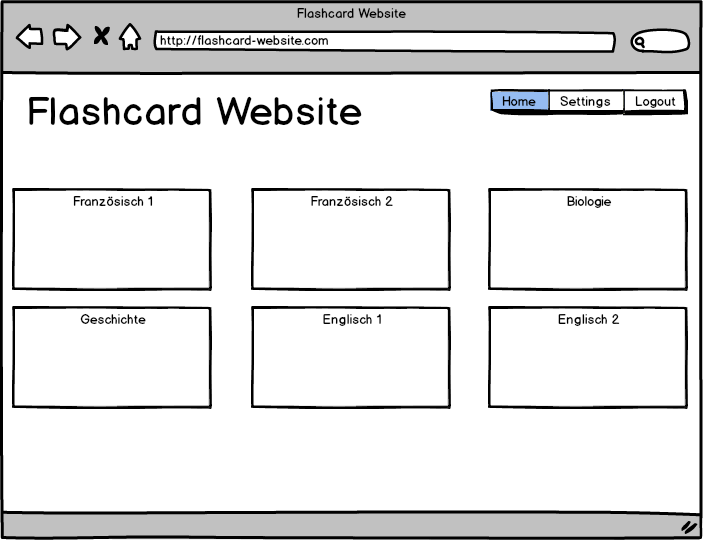
\includegraphics[width=0.7\textwidth]{images/Overview.png}
    \caption{Hauptbildschirm}
    \label{fig:overview}
\end{figure}

Der Hauptbildschirm gibt eine Übersicht zu den Karteikartensets des angemeldeten Benutzers. Beim Klicken auf eines der Sets kommt man zum Lernbildschirm


\subsubsection{Lernbildschirm}


\begin{figure}[H]
    \centering
    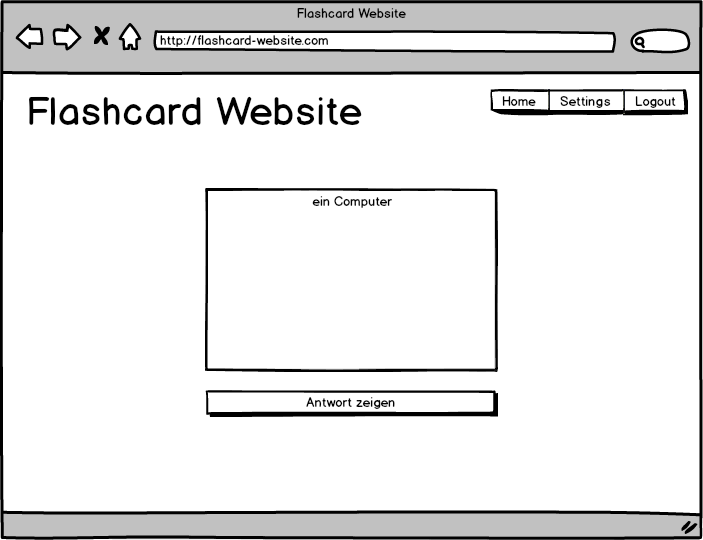
\includegraphics[width=0.7\textwidth]{images/Lernscreen-Frage.png}
    \caption{Frageseite einer Karteikarte}
    \label{fig:lernscreen-frage}
\end{figure}

\begin{figure}[H]
    \centering
    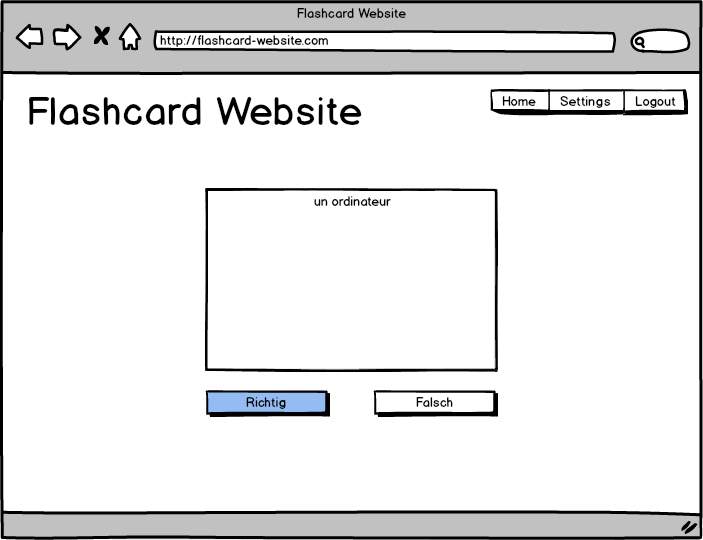
\includegraphics[width=0.7\textwidth]{images/Lernscreen-Antwort.png}
    \caption{Antwortseite einer Karteikarte}
    \label{fig:lernscreen-antwort}
\end{figure}

Der Lernbildschirm fängt mit der Vorderseite von der ersten Karteikarte des Sets an. Wenn man sich die Rückseite mit der Antwort anzeigen lässt, hat man die Möglichkeit anzugeben, ob man richtig oder falsch lag.

\begin{figure}[H]
    \centering
    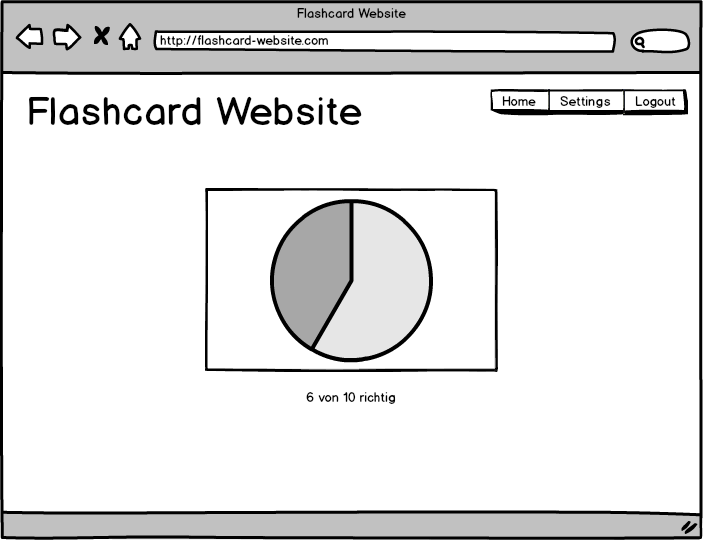
\includegraphics[width=0.78\textwidth]{images/Lernscreen-Ergebnis.png}
    \caption{Ende des Karteikartensets}
    \label{fig:lernscreen-ergbenis}
\end{figure}

\noindent Nachdem man alle Karteikarten durchgegangen ist, wird eine Statistik zu der Anzahl an richtigen Antworten angezeigt.
